\documentclass[aspectratio=43]{beamer}
\usepackage[latin1]{inputenc}
\usepackage{amsmath}
\usepackage{amsfonts}
\usepackage{amssymb}
\usepackage{makeidx}
\usepackage{graphicx}
\usepackage{array}

% Customization
\mode<presentation>{
	\usetheme{CambridgeUS}
	\usecolortheme{dolphin}
	\setbeamertemplate{navigation symbols}{}
}

% Define colors
\definecolor{darkgreen}{rgb}{0.0, 0.5, 0.13}
\definecolor{darkblue}{rgb}{0.0, 0.0, 0.55}
\definecolor{darkred}{rgb}{0.55, 0.0, 0.0}

% Title and author
\title[Perturbative QCD predictions for Higgs production]{ML and Bioinformatics}
\author{\textbf {Jes\'us Urtasun Elizari}}
%\institute{\textbf {University of Milan}}
\date{Milan, Mach 2021}

\begin{document}

% Front slide
\begin{frame}

	%\maketitle
	\vspace{1.0 cm}
	
	\center{\color{blue}Theoretical physics, Machine Learning and Bioinformatics}
	
	\vspace{0.25 cm}
	\center{Jes\'us Urtasun Elizari}
	\center{Milan, March 2021}

	\begin{figure}
		\minipage{1\textwidth}
		
\includegraphics[width = 3.0 cm]{plots/unimi.png}
		\hfill
		
\includegraphics[width = 2.5 cm]{plots/n3pdf.png}
		\hfill
		
\includegraphics[width = 3.0 cm]{plots/erc.png}
		\endminipage
	\end{figure}

	\vspace{1.0 cm}
	
	{\scriptsize \color{blue} This project has received funding from the European Union$'$s Horizon 2020 research and innovation program under grant agreement No 740006.}

\end{frame}

% Introduction
\begin{frame}

	\frametitle{Outline}
	
	\begin{enumerate}
		\item {\color{blue}QCD in a nutshell}
		\begin{itemize}
			\item The fundamental interactions
			\item Exploring matter at the small scales
			\item Hadronic physics and the LHC
		\end{itemize}
		\item {\color{blue}Machine Learning for particle physics}
		\begin{itemize}	
			\item The N3PDF project
			\item The HTurbo project
		\end{itemize}	
		\item {\color{blue}Bioinformatics}
		\begin{itemize}
			\item Applying data sciences to life sciences
		\end{itemize}
		\item {\color{blue}Summary}
	\end{enumerate}
	
\end{frame}

% QCD in a nutshell
\begin{frame}

	\center{\color{blue}Quantum Chromodynamics in a nutshell}

\end{frame}

% The Standard model
\begin{frame}
	
	\frametitle{QCD in a nutshell}
	\framesubtitle{The Standard Model}
	
	\begin{columns}

		\column{0.5\textwidth}
		
		\begin{figure}
			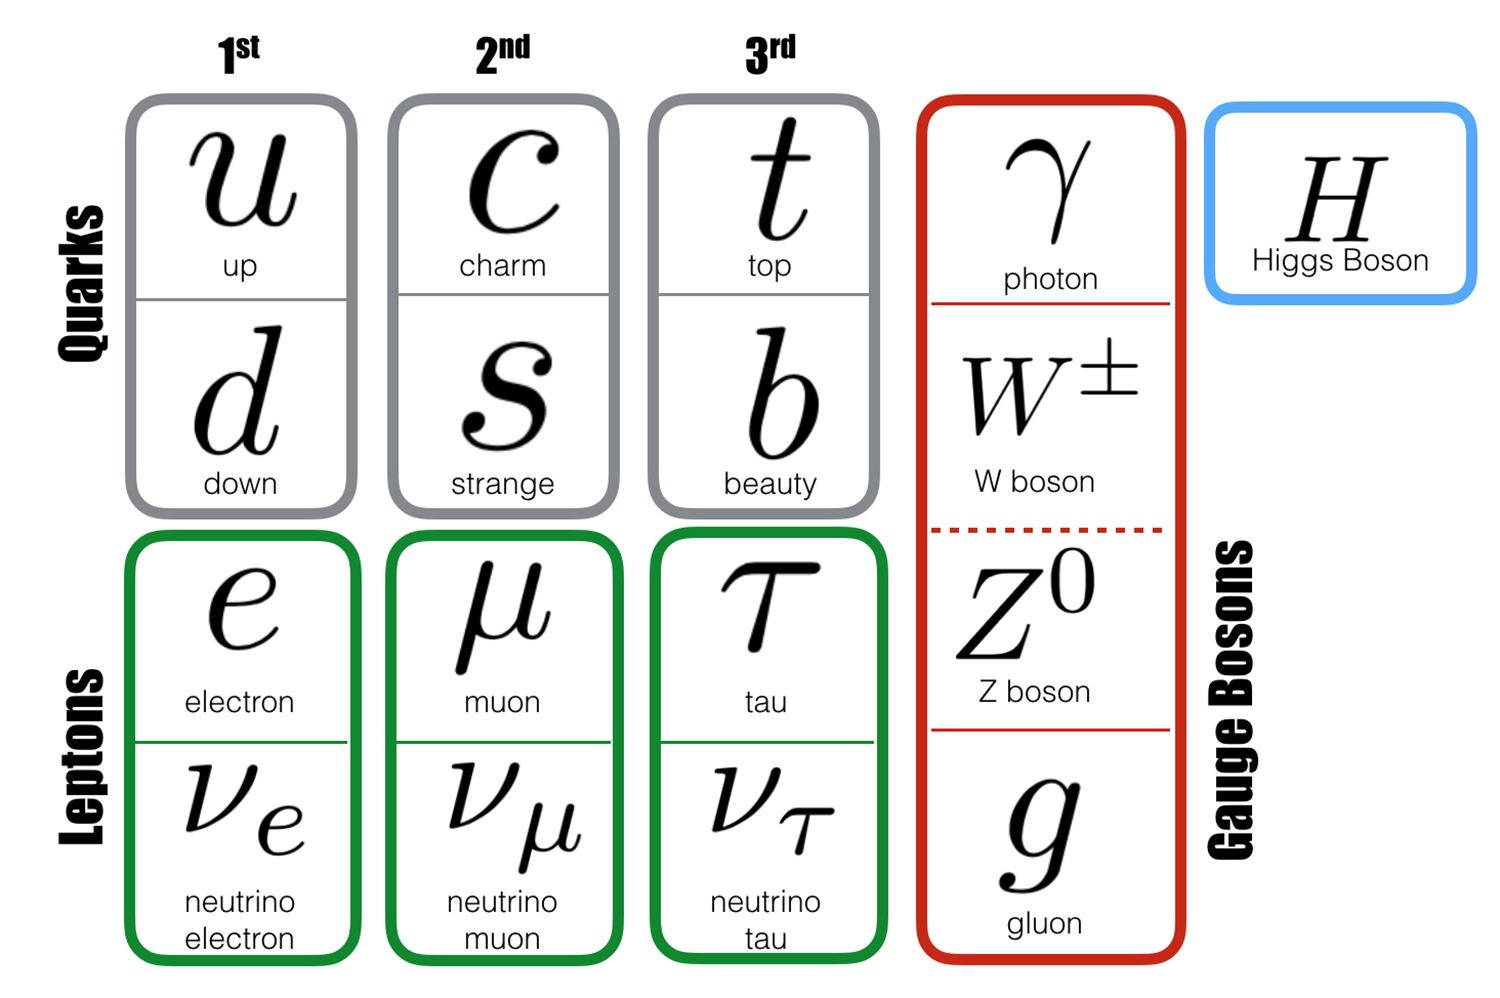
\includegraphics[width =6cm]{plots/section1/SM.png}
		\end{figure}

		\column{0.5\textwidth}
		
		\begin{figure}
			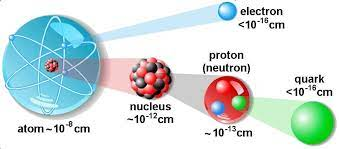
\includegraphics[width =5.75cm]{plots/section1/nucleus.jpeg}
		\end{figure}

	\end{columns}

	\vspace{0.5 cm}
		
	\footnotesize Quantum Field Theory describing physics at the TeV scale $\rightarrow$ \color{red}{less than a fermi!}
	
	\begin{enumerate}
		\item Fermions (quarks and leptons) composing matter
		\item Bosons mediating interactions
		\item Scalar Higgs field generating mass
	\end{enumerate}	

	Quantum Chromodynamics is the theory describing the strong interactions

\end{frame}

% Explore the proton structure
\begin{frame}
	
	\frametitle{QCD in a nutshell}
	\framesubtitle{Explore the strong interactions}
	
	How to explore proton's inner structure?
	
	\begin{figure}
		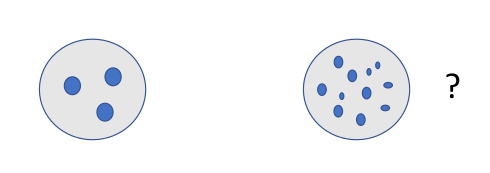
\includegraphics[width = 0.5\linewidth]{plots/section1/protons.png}
	\end{figure}
	
	
	\begin{itemize}
	\item Point-like projectile on the object $\longrightarrow$ DIS
	\item Smash the two objects $\longrightarrow$ LHC physics
	\end{itemize}
	
	{\color{blue}"A way to analyze high energy collisions is to consider any hadron as a composition of point-like constituents $\longrightarrow$ \textbf{partons"} } R.Feynman, 1969 

\end{frame}

% Parton Distribution Functions
\begin{frame}
	
	\frametitle{QCD in a nutshell}
	\framesubtitle{Parton Distribution Functions}
	
	\begin{columns}
	
		\column{0.5\textwidth}
		
		\begin{figure}
			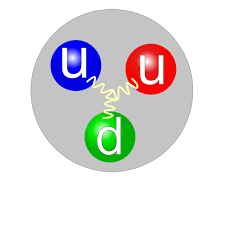
\includegraphics[width = 2cm]{plots/section1/proton.png}
		\end{figure}
		
		\column{0.5\textwidth}
	
		\begin{figure}
			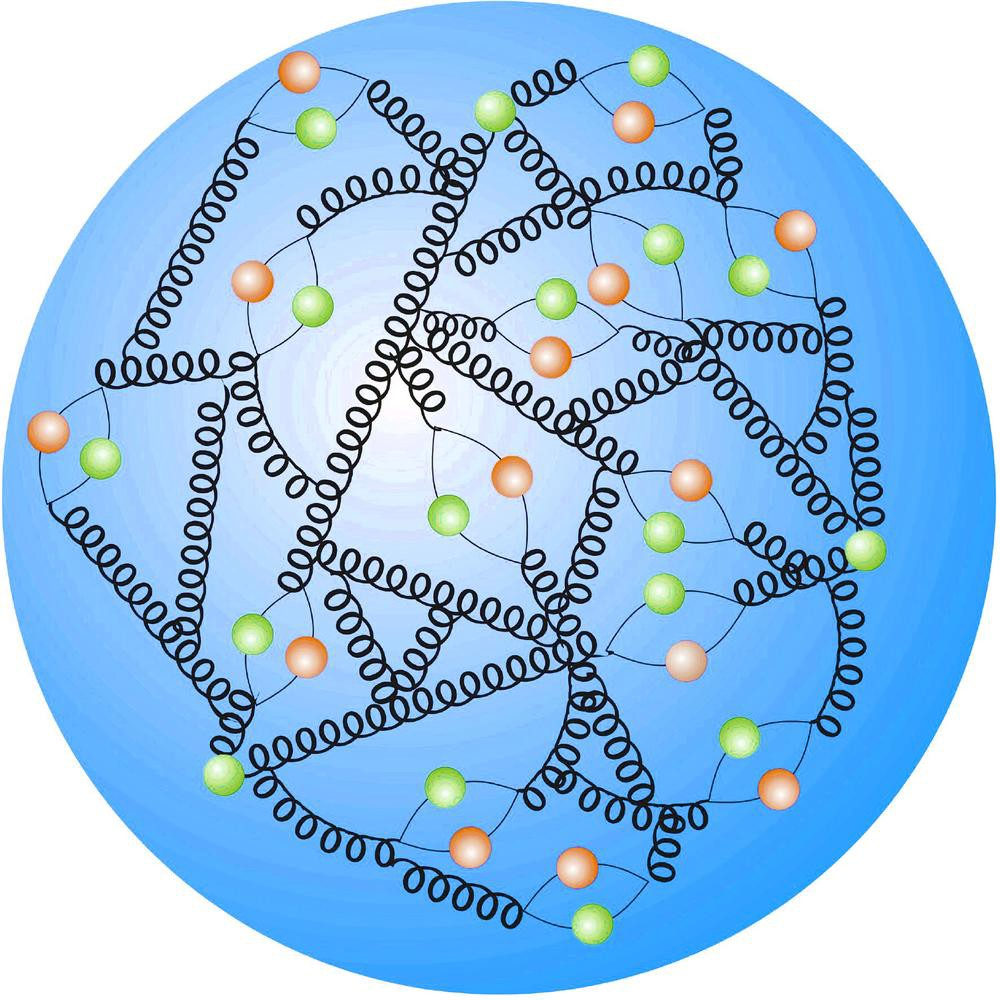
\includegraphics[width = 1.5cm]{plots/section1/proton2.jpg}
		\end{figure}
	
	\end{columns}
	
	\vspace{0.5 cm}
	
	\footnotesize
	\begin{itemize}
		\item Hadrons made of constantly interacting partons $\longrightarrow$ non perturbative physics
		\item {\color{blue}Parton distribution functions (PDFs)} are required for the precision era of the LHC
		\item PDFs can not be predicted yet not measured $\longrightarrow$ {\color{blue} extracted from data via Machine Learning algorithms}
	\end{itemize}
	
\end{frame}

% Machine Learning for particle physics
\begin{frame}

	\center{\color{blue}Machine Learning for particle physics}

\end{frame}

% Machine Learning introduction
\begin{frame}
	
	\frametitle{Machine learning}
	\framesubtitle{What is Machine Learning?}
	
	\footnotesize
	
	\begin{columns}
		
		\column{0.6\textwidth}
		
		\begin{enumerate}
			\item Machine Learning algorithms are a subset of Artificial Intelligence (AI) algorithms 
			\item Used to solve \textit{complex} tasks like classification, regression and pattern recognition
			\item Rely on comparison with data $\longrightarrow$ {\color{red}Learning}
		\end{enumerate}
		
		\column{0.4\textwidth}
		
		\begin{figure}[!htb]
			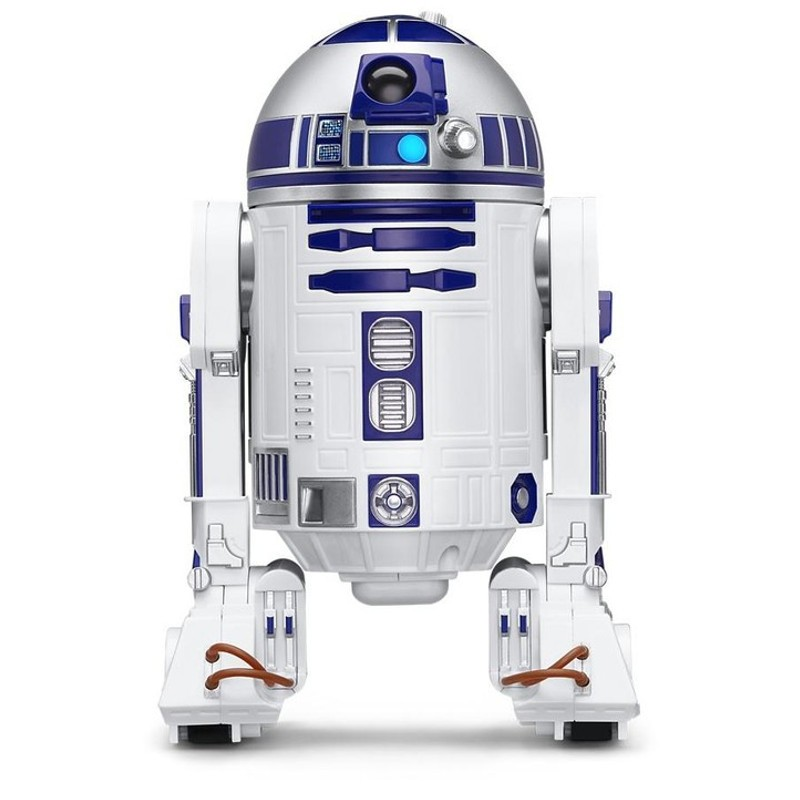
\includegraphics[width = 4cm]{plots/section2/r2d2.jpeg}
		\end{figure}
		
	\end{columns}

\end{frame}

% General structure of a fit
\begin{frame}
	
	\frametitle{The N3PDF project}
	\framesubtitle{General structure of n3fit}

	\footnotesize Parton Distribution Functions (PDFs) can not be predicted or measured\\
	{\color{red} PDFs need to be extracted from data!}

	\vspace{0.5cm}
	
	\begin{columns}
		
		\column{0.5\textwidth}
		
		
\includegraphics[width = 1.5cm]{plots/section2/TF.png}
				
		\column{0.5\textwidth}
				
		
\includegraphics[width = 2.5cm]{plots/section2/Keras.png}
		
	\end{columns}
	
	\vspace{0.5cm}
	
	\begin{itemize}
		\item \footnotesize Use TensorFlow and Keras to determine the PDFs using neural networks
		\item \footnotesize Use Stochastic Gradient Descent {\color{violet} n3fit} replacing primitive fitting algorithms
	    \item \footnotesize See paper by S.Carraza - J.Cruz-Martinez \\
		\footnotesize {\color{blue}"Towards a new generation of parton densities with deep learning models",\\ https://arxiv.org/abs/1907.05075}
		\item Operator Implementation in TF - Urtasun-Elizari et al.\\
		{\color{blue}"Towards hardware acceleration for parton densities estimation",\\ https://arxiv.org/abs/1909.10547}
	\end{itemize}

\end{frame}

% Results all
\begin{frame}
	
	\frametitle{The HTurbo project}
	\framesubtitle{Comparison HRes and HqT - all orders}

	
	\begin{figure}
		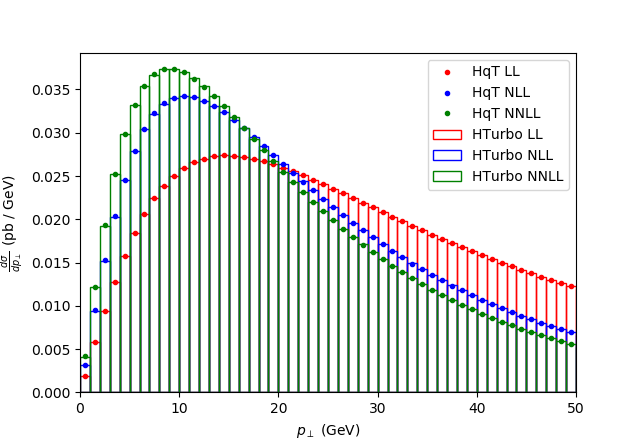
\includegraphics[width = 8cm]{plots/hturbo_all_orders.png}
	\end{figure}

	\begin{itemize}
		\item \footnotesize Older codes (\textbf{HRes}, \textbf{HqT}) need 3 days to produce NNLL distribution
		\item {\color{blue} 3 minutes with \textbf{HTurbo}!} {\color{darkgreen}$\checkmark$} 
		\item \footnotesize Agreement up to NNLL $\longrightarrow$ {\color{blue}ready for N$^{3}$LL}
	\end{itemize}

\end{frame}

% Bioinformatics
\begin{frame}

\center{\color{blue}Bioinformatics \\and \\data science for life sciences}

\end{frame}

% Bioinformatics
\begin{frame}
	
	\frametitle{Bioinformatics}
	\framesubtitle{Comoputer sciences}
	
	\begin{itemize}
		\item Python, C++, R, Machine Learning
		\item {\color{blue}[https://github.com/JesusUrtasun/CppCourse]}
		\item {\color{blue}[https://github.com/JesusUrtasun/MLcourse]}
		\item {\color{blue}[https://github.com/JesusUrtasun/Bioinformatics]}
	\end{itemize}

\end{frame}

% Bioinformatics
\begin{frame}
	
	\frametitle{Bioinformatics}
	\framesubtitle{DNA and RNA sequencing data}
	
	\begin{itemize}
		\item Processing and data grooming of DNA and RNA sequencing data
		\item Statistics and data analysis of BAM files with R
		\item \textbf{Rsubred} and \textbf{Dseq2} packages
		\item \color{blue} Fast learner!
	\end{itemize}

\end{frame}

% Conclusions
\begin{frame}
	
	\frametitle{Summary $\&$ Conclusions}

	\vspace{2.0 cm}
	
	\begin{enumerate}
		\item \footnotesize Precise knowledge of sub-nuclear interactions are required towards the precision era of the LHC
		\item \footnotesize Machine Learning models provide a robust way for PDFs determination optimized through {\color{blue}operator implementation in TF}
		\item \footnotesize We develop a numerical code \textbf{HTurbo}, implementing $q_{\perp}$ resummation for Higgs boson production, which is {\color{blue} faster than any of the existing codes}
		\item \footnotesize Experience with Python and R for NGS data, and still looking to improve!

	\end{enumerate}

	\vspace{2.0 cm}

\end{frame}

% Conclusions
\begin{frame}

	\center \footnotesize {\color{blue}Thank you!}

	\begin{figure}
		
\includegraphics[width = 2.5 cm]{plots/thinking.png}
	\end{figure}		

\end{frame}


% Factorization theorem
\begin{frame}
	
	\frametitle{Back up}
	\framesubtitle{Hadronic collisions}
	
	\center \textrm{Hadronic Physics} \footnotesize $h_{1}(p_{1}) + h_{2}(p_{2}) \rightarrow F + X$ 
	
	\begin{figure}
		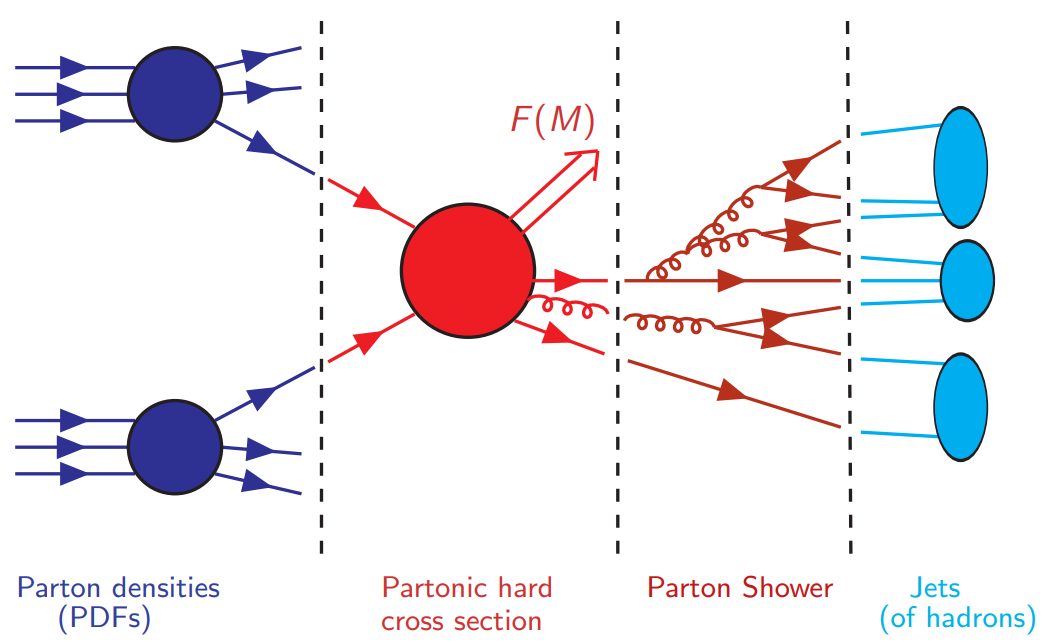
\includegraphics[width = 7 cm]{plots/section1/factorization_1.png}
	\end{figure}
	
	\center \footnotesize {Factorize process as {\color{blue}PDFs} and {\color{red} partonic (hard) interaction}	
	\begin{equation}
		\sigma^{\textrm{F}}(p_{1}, p_{2}) = \sum_{\alpha, \beta}
		\int_{0}^{1} dx_{1} dx_{2} \; {\color{blue} f_{\alpha/h_{1}}(x_{1}, \mu_{F}^{2}) \ast f_{\beta/h_{2}}(x_{2}, \mu_{F}^{2})}
		\; \ast \;  
		{\color{red}\hat{\sigma}^{\textrm{F}}_{\alpha \beta}(x_{1}p_{1}, x_{2}p_{2}, \alpha_{s}(\mu_{R}^{2}), \mu_{F}^{2})} \nonumber
	\end{equation}}

\end{frame}

% The N3PDF project
\begin{frame}

\frametitle{Back up}
\framesubtitle{Operator implementation in TF}

\begin{figure}
	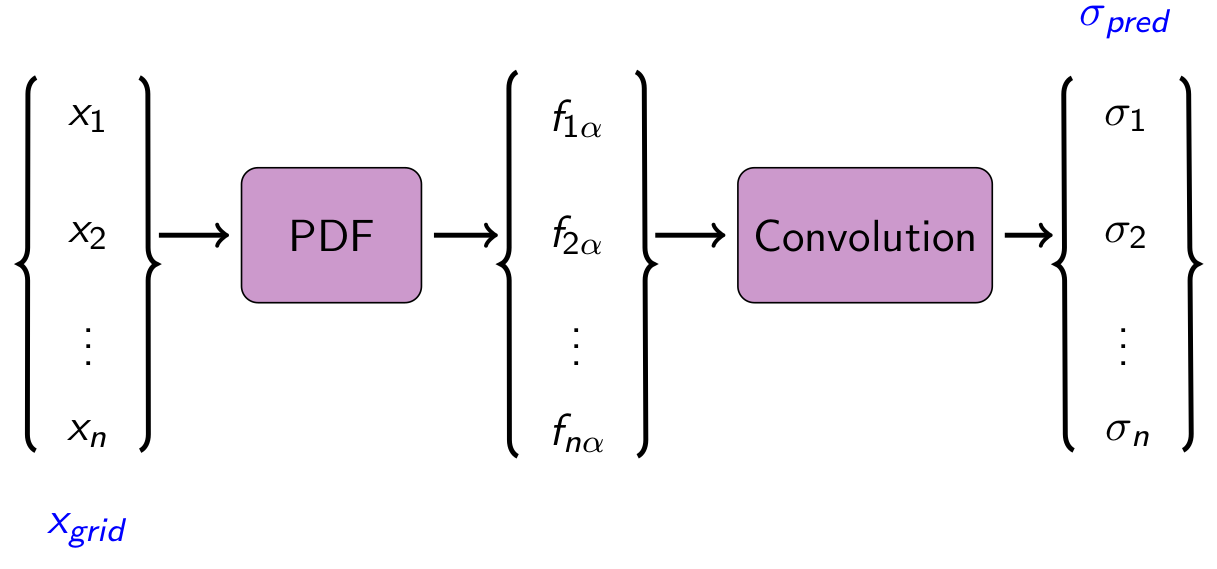
\includegraphics[width = 8.5 cm]{plots/section2/TF_convolution.png}
\end{figure}


\begin{itemize}
	\item \footnotesize Build a NN model to compute $\sigma_{pred}$ observables from a grid $x_{i}$
	\item \footnotesize Perform $\chi^{2}$ minimization comparing with data
	\item \footnotesize Update values of PDF $\longrightarrow$ {\color{violet} Fit}
\end{itemize}

\end{frame}

% The N3PDF project
\begin{frame}

\frametitle{The N3PDF project}
\framesubtitle{Operator implementation in TF}

\begin{figure}
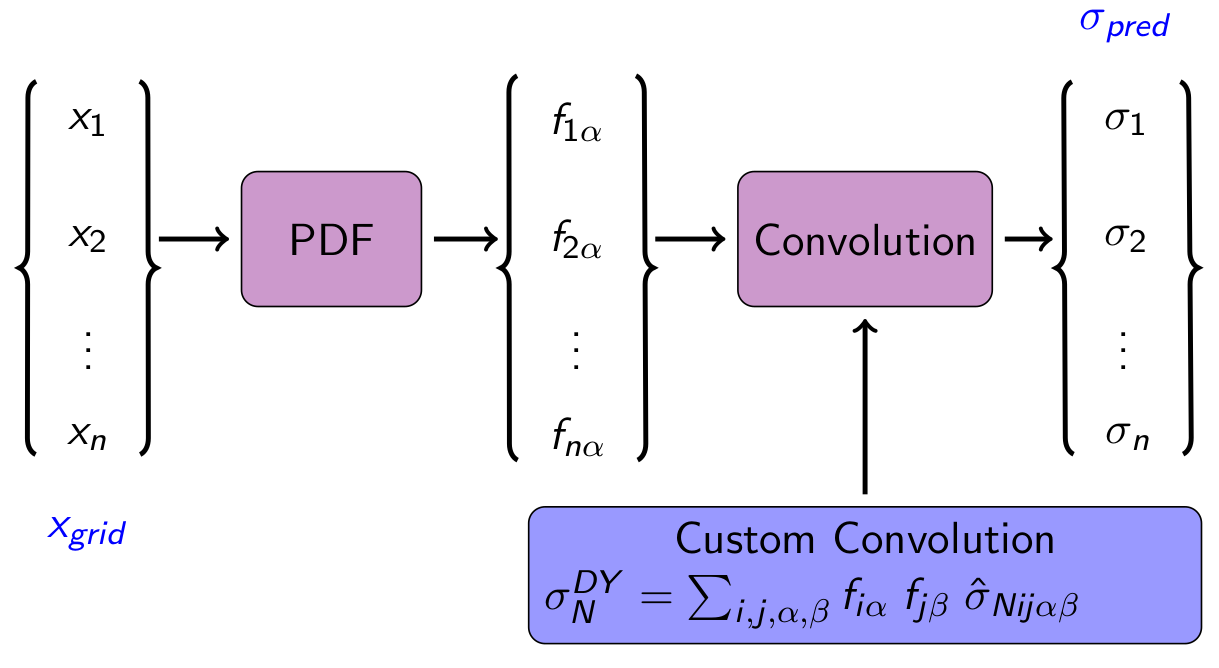
\includegraphics[width = 8.5 cm]{plots/section2/TF_convolution2.png}
\end{figure}

\begin{enumerate}
\item \footnotesize TF relies in symbolic computation $\longrightarrow$ High memory usage
\item \footnotesize Implement c++ operator replacing the convolution
\item Further details in Urtasun-Elizari et al.\\
{\color{blue}"Towards hardware acceleration for parton densities estimation",\\ https://arxiv.org/abs/1909.10547}
\end{enumerate}

\end{frame}

\end{document}